\setAuthor{Jaan Kalda}
\setRound{lõppvoor}
\setYear{2022}
\setNumber{G 1}
\setDifficulty{1}
\setTopic{TODO}

\prob{Kettaheide}
Taganttuul on spordis harilikult abiks, kuid mitte kettaheites. Selgitage kvalitatiivselt, miks vastutuul võib suurendada kettaheite tulemust. Visandage joonis, kus lendav ketas on kujutatud vertikaalläbilõikes näidates seal ketta lennusuuna ja tuule suuna. Näidake sellel joonisel jõudiagrammina, millised jõud mõjuvad kettale lennu ajal ja kirjeldage, kuidas mõjutab neid jõude vastutuul.


\hint

\solu
\

\begin{figure}[h]
    \centering
    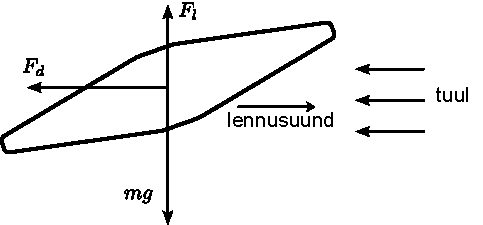
\includegraphics[]{2022-v3g-01-sol.pdf}
\end{figure}

Jõudiagramm on toodud joonisel. Vastutuul suurendab nii takistusjõudu kui õhuvoolust tingitud üleslükkejõudu. Üleslükkejõud kasvab proportsionaalselt ketta kiirusega õhu suhtes. Suurem üleslükkejõud pikendab lennuaega, mille tulemusel jõuab ketas liikuda horisontaalsihis kaugemale vaatamata sellele, et horisontaalsuunaline kiirus natuke väheneb takistusjõu tõttu (esimene efekt on tugevam, kui teine).
\probend